\chapter{Methodology}

We evaluate the performance of an available ICN 
implementation --- Project CCNx~\cite{website:ccnx}\,\footnote{We henceforth 
address the CCN networking concept as `CCN' and its implementation as `CCNx'.} --- 
by setting up a simple testbed, composed by commercial off-the-shelf (COTS) 
equipment. Besides validating some of the claims made by CCN, we attempt to 
compare CCNx applications to equivalent `host centric' solutions.\vertbreak

This section (1) describes the CCNx software 
package to be used in the tests, (2) provides an overview of the testbed's 
structure and (3) details the protocol of the tests to be conducted.

\section{Project CCNx}

Project CCNx~\cite{website:ccnx} provides an open source software reference 
implementation PARC's CCN architecture~\cite{Jacobson2009}, with the 
objective of enabling experimentation in the network research community. The 
project provides APIs written in multiple programming languages (C, Java and 
Android), with extensive documentation.\vertbreak

CCNx is designed to run on top of 
existing transport protocols and addressing schemes --- TCP, UDP, 
etc. --- in an `overlay' approach. This means that CCNx packets are tunneled 
within TCP or UDP flows running over IP. Although Project CCNx developers 
present this as a short-term approach for developers to start trying 
CCN, it is also presented as a feature, implying CCN's advantage over similar 
solutions in the current networking paradigms (e.g. web 
caching)~\cite{Jacobson2009,website:ccnx,Willis2012,Melazzi2012}.

\subsection{CCNx Applications}

Project CCNx 
provides the following ensemble of example applications~\cite{Muther2012a}:

\begin{itemize}

    \item \verb?ccnchat?: Simple application for real-time transmission of text 
            messages from sender to receiver.
    \item \verb?ccnfileproxy?: Allows one to share files within the 
            node's file system to other CCNx 
            nodes\textsuperscript{\ref{foot:note1}} (used as an alternative to 
            setting up a CCNx repository~\cite{Muther2012a}).
    \item \verb?ccnputfile?\,\slash\,\verb?ccngetfile?: Pair of applications to 
            write\slash read files to\slash from CCNx nodes, e.g. to store 
            files into a CCNx repository.
    \item \verb?ccnsendchunks?: Simple application 
            which divides a given piece of content in `chunks' upon the 
            reception of Interest packets directed at that same content, and 
            sends the `chunks' as Data packets towards the requester. Interest 
            packets are generated via the complementing \verb?ccncatchunks2?
            application.
    \item VLC CCNx plugin: Plugin to the VLC media player~\cite{website:vlc}, 
            which allowing a CCNx node to remotely playback a video stored on a 
            CCNx repository, identified by its `content name'.
    \item Others (see Section `What To Look At' in~\cite{Muther2012a}).

\end{itemize}

The diversity of application types listed above may translate into a reasonably 
sized set of test possibilities. However, their specific CCNx implementations may 
significantly differ from those one would use in the non-CCNx case (e.g. 
\verb?ccnchat? vs. an established instant messaging application 
or protocol e.g. XMPP). The influence of implementations should be taken 
into account when analyzing network performance results.\vertbreak

\subsection{Specificities of CCNx Applications}
\label{subsec:ccnx-specifics}

Here we provide CCNx application-specific information, useful for understanding the 
tests and results shown in later sections.

\subsubsection{CCNx Forwarding Tables}
\label{subsubsec:fibs}

Since CCNx works as an `overlay', CCN's routing scheme based on content must be 
translated into IP routing at a given point. In CCNx this is accomplished 
by the routing daemon, \verb+ccnd+, the main process running in CCNx 
nodes~\cite{website:ccnx-commands}.\vertbreak

As dynamic routing in CCNs is still an area of current research 
and not well supported by current CCNx releases~\cite{Wang2012,Hoque:2013:NNL:2491224.2491231}, 
we adopt the same strategy as that applied in previous work~\cite{Wahlisch2012, Vahlenkamp2012} 
and manually added static routes to CCNx's Forwarding Table (FIB), using the 
\verb+ccndc+ utility~\cite{website:ccnx-commands}. We provide examples of 
the \verb+ccndc+ command in Appendix~\ref{app:ccnx-specificss}.

\subsubsection{Disseminating Content with CCNx}
\label{subsubsection:disseminating-ccnx}

In CCNx, content sources use a specific repository application for storing 
content and make it available in CCNx networks by responding to 
matching Interests, \verb+ccnr+~\cite{website:ccnx-commands}. The \verb+ccngetfile+ application~\cite{website:ccnx-commands} 
can then be used to release Interest packets to the CCNx network, querying 
for particular content. Appendix~\ref{app:ccnx-specificss} presents some concrete examples 
of the usage of these applications.\vertbreak

CCNx also provides \verb+ccnsendchunks+ and \verb+ccncatchunks2+, another duet 
of applications for content exchange. \verb+ccnsendchunks+ takes content (e.g. 
a file) as input, and produces Data packets containing `chunks' of the content 
(blocks of a given size, in byte) as it receives Interests, or at a rate of 
one-per-second, whichever is faster\,\footnote{Although no 
MAN page exists for this command, the following resource may be used as an unofficial 
source of information: \url{https://www.ccnx.org/pipermail/ccnx-dev/2010-April/000189.html}.}. 
The complementary Interest-producing \verb+ccncatchunks2+ also uses pipelining 
of Interests, varying 
its `window size' according to the rate of arrival of Data packets. This 
behavior is also analyzed in some of the tests specified in 
Section~\ref{sec:protocol}. We provide examples of the use 
of both commands in Appendix~\ref{app:ccnx-specificss}.\vertbreak

Video content stored in a CCNx repository may be directly played back in 
VLC media player~\cite{website:vlc}, using a special CCNx plugin which 
generates Interests for that content (any type of content playable by VLC, 
e.g. a \verb+.avi+ file), receives the respective Data packets, decodes them 
and progressively plays them back. Again, we provide examples of its 
usage in Appendix~\ref{app:ccnx-specificss}.

\section{Testbed Description}
\label{sec:testbed}

The basic testbed structure used for evaluation of CCNx is depicted in 
Figure~\ref{fig:basic-testbed}. Some tests require alterations to this scheme, 
nevertheless such alterations are promptly indicated 
in the individual test descriptions, in Section~\ref{sec:protocol}. Table~\ref{tab:hw} 
provides a list with more details of the testbed equipment.\vertbreak

\begin{figure}[h!]

    \centering
    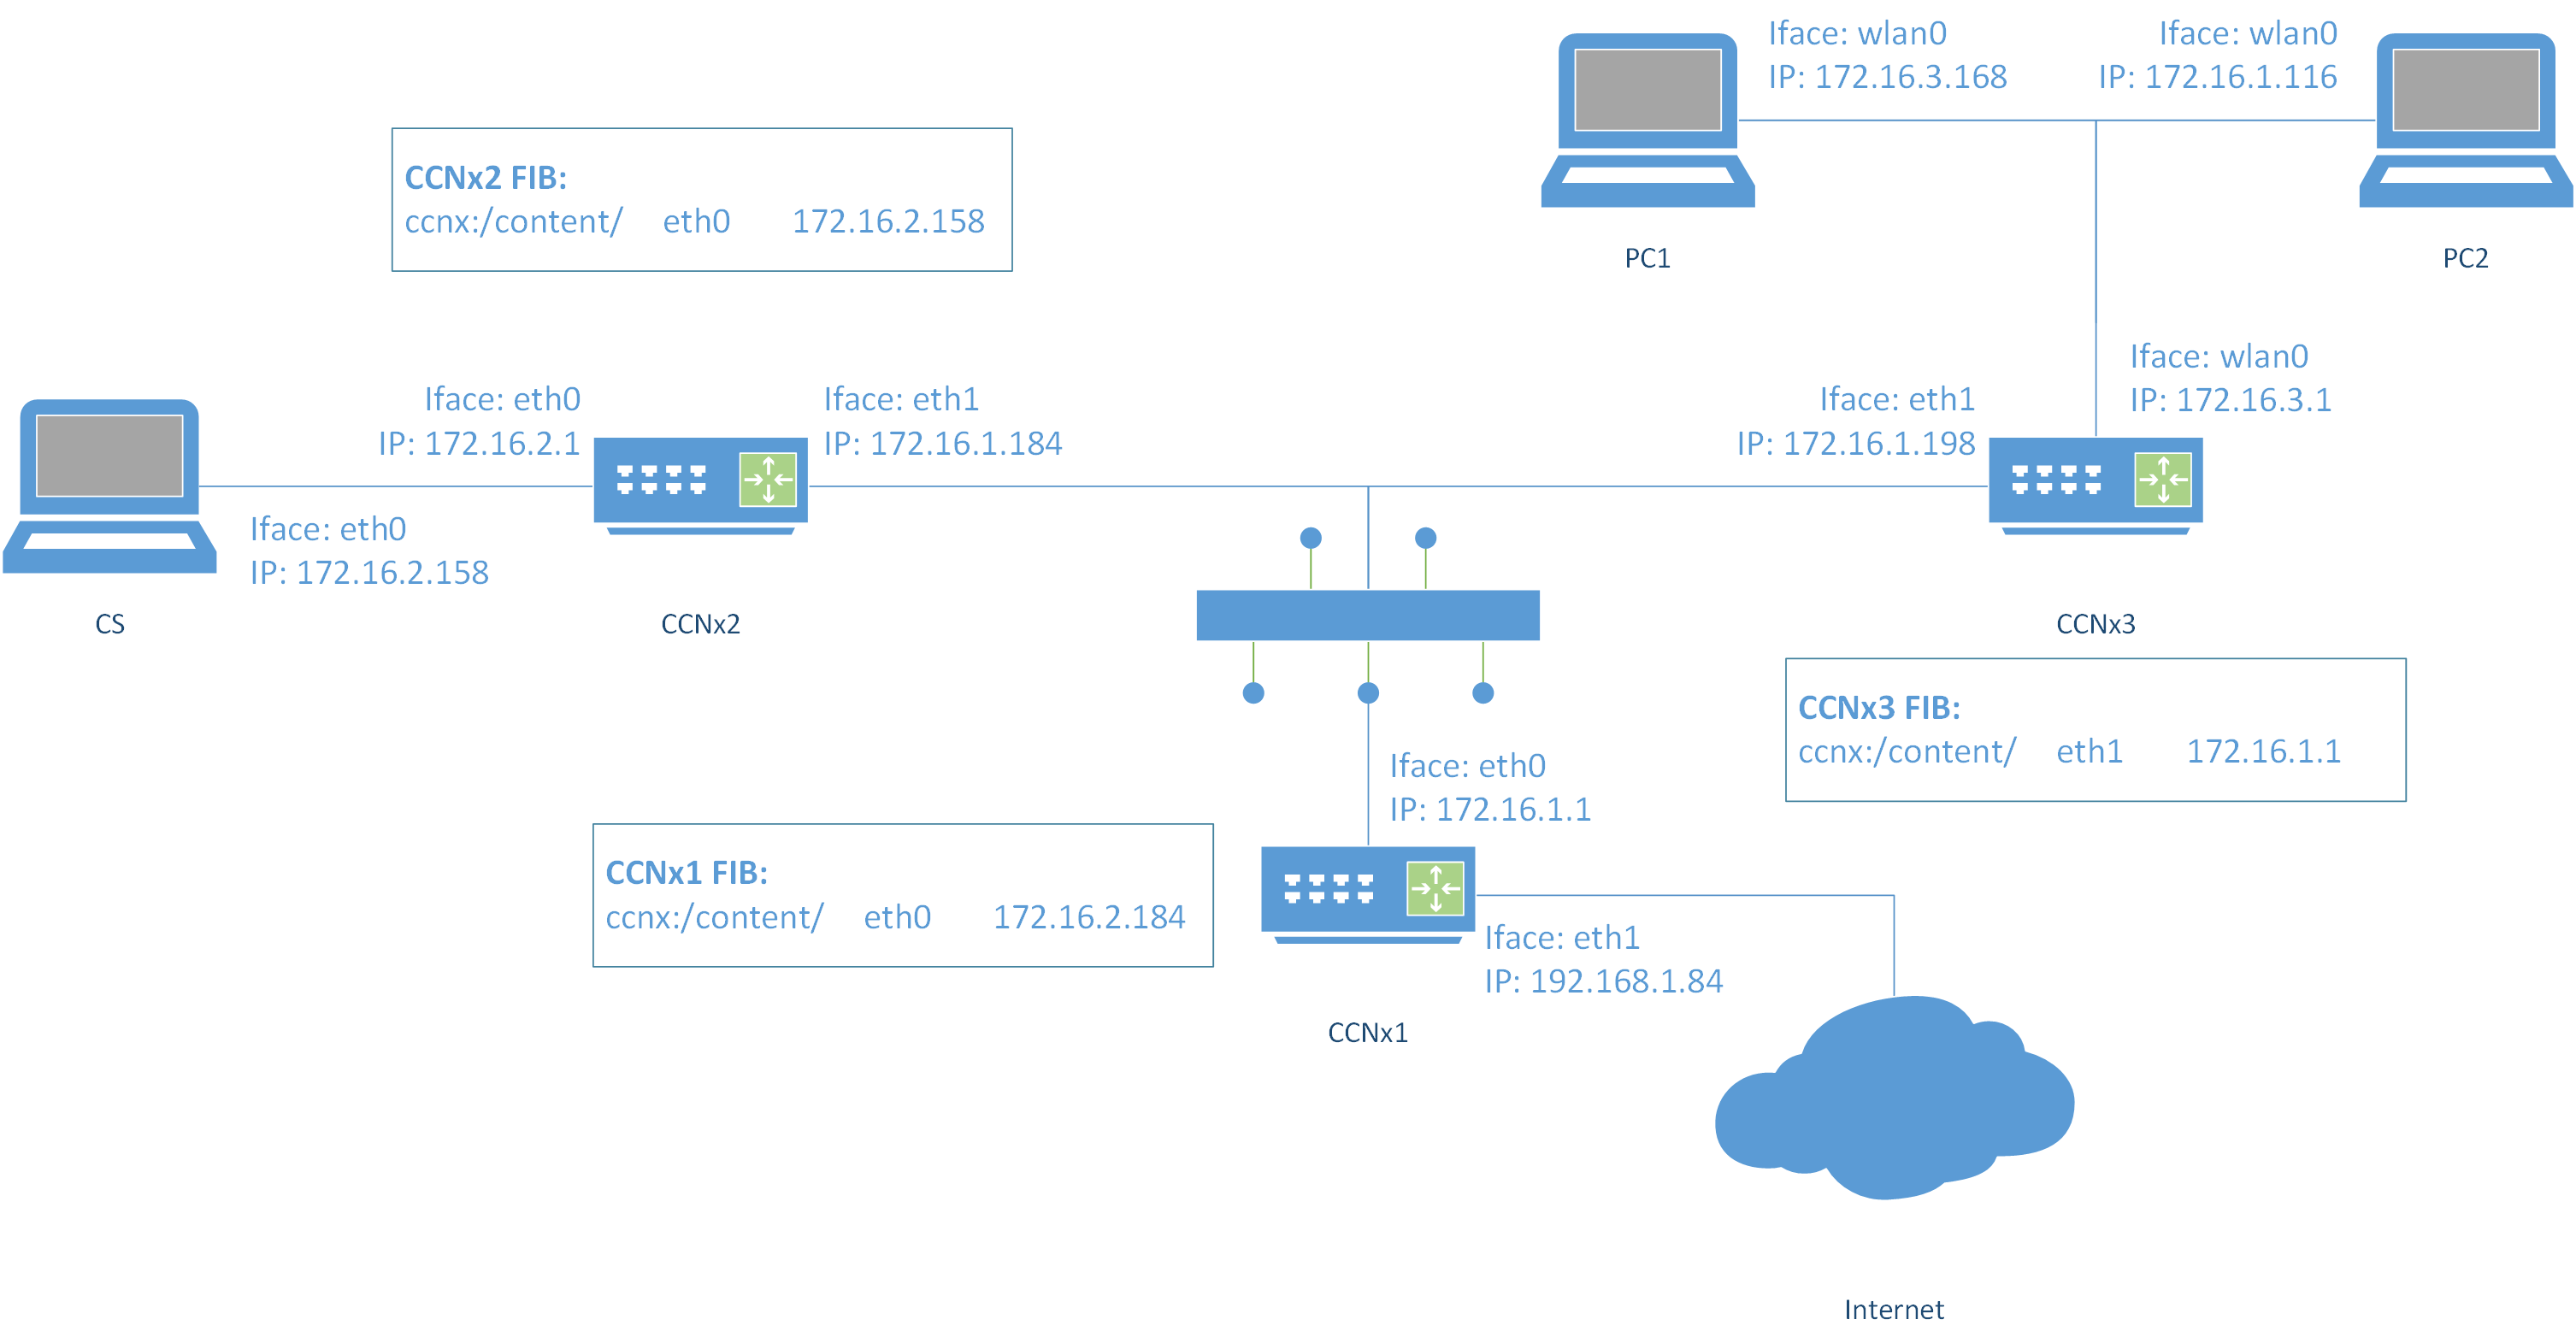
\includegraphics[width=0.80\textwidth]{figures/diag1.png}
    \cprotect\caption{Basic arrangement for the proposed testbed.}
    \label{fig:basic-testbed}

\end{figure}

The basic scenario depicted above includes 3 COTS residential routers, labeled 
as `CCNx1', `CCNx2' and `CCNx3' (Linksys WRT160NL) running OpenWRT\,\footnote{`Barrier 
Breaker' version, SVN revision 35323, available at \url{https://dev.openwrt.org/browser/trunk?rev=35323}.}~\cite{website:openwrt}, a Linux-based 
operating system. These represent the Inner Nodes (INs) of a network, 
serving as CCNx\slash IP routers (see Section~\ref{subsubsec:ccnx-openwrt} for details on the 
installation of CCNx software on embedded Linux systems). Table~\ref{tab:hw} 
summarizes the hardware specifications of these devices.\vertbreak 

The arrangement 
separates the End Nodes (ENs) --- consumers of content --- and the Content 
Sources (CSs) --- generators of content --- in different 
IP subnets (172.16.x.x), so that routing is performed in both CCNx and `host centric' 
scenarios\,\footnote{As CCNx works as an overlay, IP routing will be performed 
in both CCNx and `host centric' test versions. Nevertheless, as this work may 
potentially origin subsequent research (e.g. testing dynamic routing in CCNx), 
we believe it is good practice to test this scenario from the start}.\vertbreak

\begin{table}[h!]
    \centering
    \footnotesize
        \begin{tabularx}{1.00\textwidth}{ l l X X c }
            %\hline
            \toprule
            \textbf{Test Element} & \textbf{Label(s)} & \textbf{Type} & \textbf{Relevant Specs.}  & \textbf{Qty.} \\ [0.5ex]
            \midrule
            \multirow{2}{*}{Content Source(s)} & \multirow{2}{*}{CS} & \multirow{2}{*}{Laptop (w\slash Ubuntu 12.04)} & Wi-Fi: 802.11 b/g & \multirow{2}{*}{1} \\ [0.5ex]
                                               & & & Ethernet: 10\slash 100\,Mbps & \\ [0.5ex]
\midrule
            \multirow{4}{*}{Inner Node(s)}  & CCNx1 & \multirow{4}{*}{Linksys WRT160NL~\cite{website:wrt160nl}} & CPU: Atheros 9130-BC1E 400 Mhz    & \multirow{4}{*}{3} \\ [0.5ex]
                                            & CCNx2 &              	& RAM: 32 MB                        & \\ [0.5ex]
                                            & CCNx3 &               & Wi-Fi: 802.11 b/g/n               & \\ [0.5ex]
                                            & &                     & Ethernet: 10\slash 100\,Mbps      & \\ [0.5ex]
            \midrule
            \multirow{2}{*}{End Node(s)}    & PC1   & \multirow{2}{*}{Laptop (w\slash Ubuntu 12.04)}    & Wi-Fi: 802.11 b/g/n & \multirow{2}{*}{2} \\ [0.5ex]
                                            & PC2   &                                                   & Ethernet: 10\slash 100\,Mbps      & \\ [0.5ex]
            \bottomrule
        \end{tabularx}
    \caption{Table of hardware for the testbed depicted in Figure~\ref{fig:basic-testbed}.}
    \label{tab:hw}
\end{table}

\subsection{Testbed Setup Details}

%This section documents pertinent notes about the testbed setup process, 
%specifically related to the installation of CCNx at the network nodes.

\subsubsection{Setting up CCNx at End Nodes (ENs)}

We have used the latest release of CCNx (0.8.1)\,\footnote{Compiled from source, 
available at \url{http://www.ccnx.org/software-download-information-request/download-releases/}} at the EN nodes. 
In addition to the basic CCNx package, the VLC plugin (available with CCNx 0.8.1 package)
was separately compiled and installed at the ENs, in order test dissemination 
of video content in CCNx networks. The VLC version 2.0.8 TwoFlower was used 
for testing at the ENs.\vertbreak

As the objective of the work is to monitor the performance of CCNx according to 
network parameters such as network load, throughput, latency, etc. a patched 
version of Wireshark (version 1.8.6) was re-compiled to include a CCN packet 
dissector~\cite{website:ccn-wireshark}.

\subsubsection{Setting up CCNx at Inner Nodes (INs)}
\label{subsubsec:ccnx-openwrt}

Testing CCNx on `real-world' constrained devices was a clear 
intention of this work, making it different from other 
studies (e.g. Vahlenkamp et 
al.~\cite{Wahlisch2012, Vahlenkamp2012}). Although no CCNx packages were 
directly available to OpenWRT, a custom OpenWRT build with a CCNx 
package~\cite{website:ccn-openwrt} (version 0.7.2) designed for a different 
distribution --- CeroWRT~\cite{website:cerowrt} --- was successfully 
accomplished. 

%Refer to Appendix~\ref{app:openwrt-ccnx-build} for details on 
%the process followed for building an OpenWRT image with CCNx.

\section{Test Specification}
\label{sec:protocol}

The following subsections describe the set of tests to perform over the 
base testbed shown in Section~\ref{sec:testbed}. A summary of the test setups 
is given in Table~\ref{tab:tests}.

\begin{table}[H]
    \centering
    \begin{threeparttable}
    \footnotesize
        \begin{tabularx}{1.00\textwidth}{ c l l X l }
            %\hline
            \toprule
            \textbf{Number} & \textbf{Applications} & \textbf{Parameters} & \textbf{Testbed Configs.} & \textbf{Descr.}\\ [0.5ex]
            \midrule
            \multirow{3}{*}{1} & \multirow{3}{*}{File transfer} & Throughput & \multirow{3}{*}{Fig.~\ref{fig:test-1-1}} & Simple file transfer between two ENs.\\ [0.5ex]
                & & Qty. packets\slash byte & \\ [0.5ex]
                & & Other                   & \\ [0.5ex]
            \midrule
            \multirow{3}{*}{2.1} & \multirow{3}{*}{File transfer} & Network load & \multirow{3}{*}{Fig.~\ref{fig:basic-testbed}} & File transfer with CCNx multihop forwarding.\\ [0.5ex]
                & & Qty. packets\slash byte & & \\ [0.5ex]
                & & CPU and RAM usage       & & \\ [0.5ex]
            \midrule
            \multirow{3}{*}{2.2} & \multirow{3}{*}{Video Streaming} & Network load & \multirow{3}{*}{Fig.~\ref{fig:basic-testbed}} & Video streaming under multihop forwarding.\\ [0.5ex]
                & & Qty. packets\slash byte & & \\ [0.5ex]
                & & CPU and RAM usage       & & \\ [0.5ex]
            \midrule
            \multirow{3}{*}{2.3} & \multirow{3}{*}{File Transfer} & Network load & \multirow{3}{*}{Fig.~\ref{fig:testbed-multiple-paths}} & CCNx multihop forwarding with multiple paths.\\ [0.5ex]
                & & Qty. packets\slash byte & & \\ [0.5ex]
                & & CPU and RAM usage       & & \\ [0.5ex]
            \bottomrule
        \end{tabularx}
        %\begin{tablenotes}
            %\footnotesize
        %\end{tablenotes}
    \caption{Summary of the tests to be ran on the testbeds depicted 
        in Figures~\ref{fig:basic-testbed},~\ref{fig:test-1-1}, and~\ref{fig:testbed-multiple-paths}.}
    \label{tab:tests}
    \end{threeparttable}
    %\end{center}
\end{table}

\subsection{Test 1 - CCNx Throughput and Overhead}
\label{subsec:test-throughput-overhead}

The objective of this test is to assess CCNx throughput and overhead by monitoring 
the exchange of content between two ENs (PC1 and CS) using 
\verb+ccnsendchunks+ and \verb+ccncatchunks2+. In this case, a 
simpler scheme than that shown in Figure~\ref{fig:basic-testbed} is used, 
depicted in Figure~\ref{fig:test-1-1}.\vertbreak

\begin{figure}[h!]

    \centering
    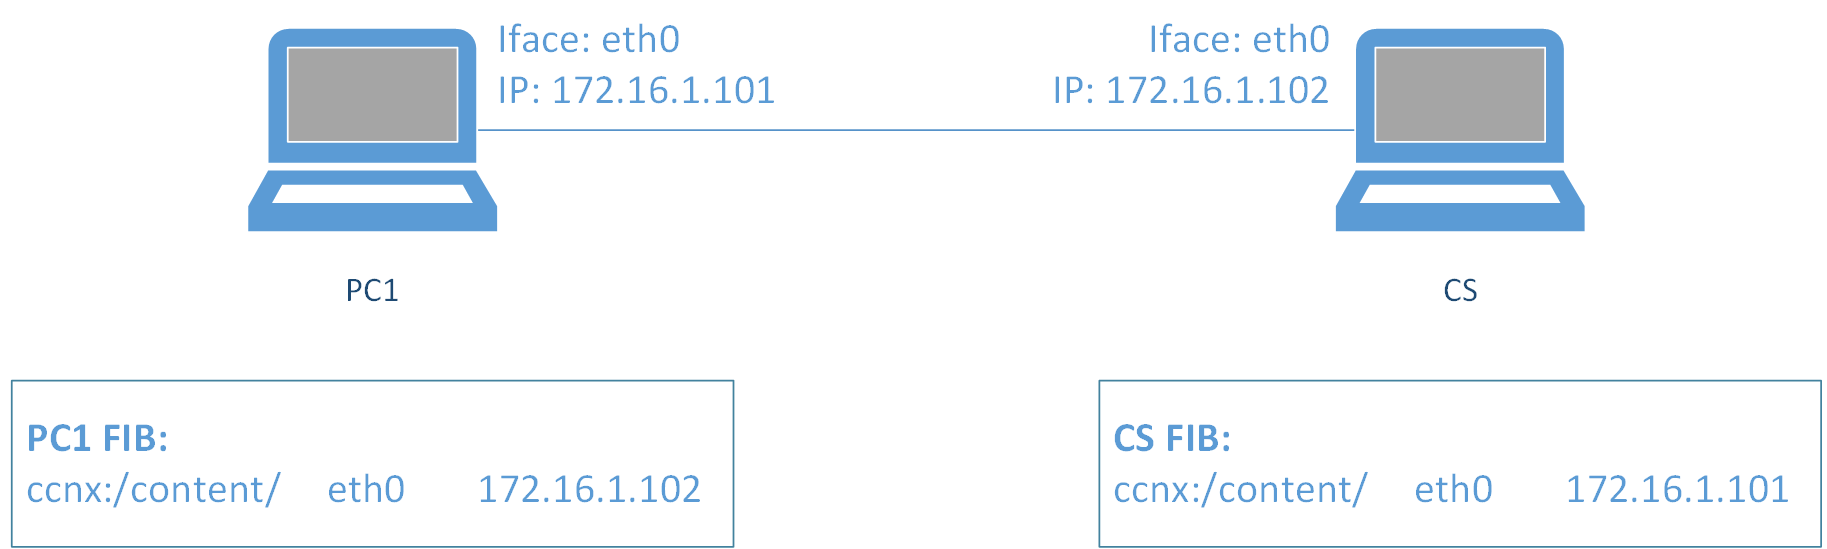
\includegraphics[width=0.80\textwidth]{figures/diag3.png}
    \cprotect\caption{Example of the configuration for Test 1. PC1 shall 
            execute \verb?ccncatchunks?, while CS executes \verb?ccnsendchunks?.}
    \label{fig:test-1-1}

\end{figure}

As \verb+ccncatchunks2+ implements its own flow control mechanism, the FIBs of 
both CCNx nodes are configured to route packets over UDP (see 
Section~\ref{subsubsec:fibs} for details), in order to avoid interference 
from TCP's own flow control. The content used for 
exchange in the tests consists in randomly generated data files of 500\,kB, 
5\,MB and 50\,MB. The chunk size parameter of \verb+ccnsendchunks+ is tested 
under three different values: 1024 byte, 4096 byte and 8192 byte.\vertbreak

The following parameters are measured:

\begin{enumerate}
    \item Throughput;
    \item Number of packets exchanged between ENs, discriminated by type;
    \item Bytes exchanged between ENs;
    \item Other parameters specific to \verb+ccncatchunks2+ flow control 
        mechanism.
\end{enumerate} 

Parameters 1, 2 and 3 from the above list shall be measured on a non-CCNx 
setting, by transferring data over FTP. The same setup shown 
in Figure~\ref{fig:test-1-1} is used, with CS running an FTP server 
(\verb?proftpd?\,\footnote{Available at \url{http://www.proftpd.org/}}) and PC1 
fetching content using an FTP client. Again, the content to be exchanged in the 
tests consists in the same randomly generated data files used in the CCNx tests.\vertbreak

\subsection{Test 2.1 - CCNx Multihop Forwarding (File Transfer)}
\label{subsec:test-multihop-file}

Here we test CCNx on the testbed scenario depicted in 
Figure~\ref{fig:basic-testbed}. The objective is to monitor network parameters as 
CCNx routers (INs) forward Interest and Data packets to\slash from a content source (CS) and 
two content consumers (PC1 and PC2), both sending Interests for the same 
content.\vertbreak

The same type of content as that used in Test 1 is used, but 
limited to a 5\,MB file\,\cprotect\footnote{\label{foot:note1}Preliminary tests with larger files (e.g. 50\,MB) 
have been conducted, however since \verb+ccnd+ keeps its cache in memory and 
due to issues in the cache replacement mechanism of OpenWRT's \verb+ccnd+, the 
RAM of the Linksys WRT160NL would exhaust quickly forcing a system restart.}. 
In this case, the \verb+ccnr+ application is used at CS to host a CCNx file 
repository, while PC1 and PC2 retrieve the file using \verb+ccngetfile+. Two 
subtypes of test are conducted: (1) PC1 and PC2 start the 
file transfer separately in time, i.e. PC2 starts releasing Interest packets 
after PC1 receives its last Data packet; and (2) PC1 and PC2 content 
requests overlap. The integrity of the transmitted files is verified via an 
MD5 checksum, for all transfers.\vertbreak

The following parameters are measured:

\begin{enumerate}
    \item Network load (packets\slash sec) at the different interfaces of INs, over time;
    \item Number of packets exchanged between INs, discriminated by type;
    \item Bytes exchanged between INs;
    \item CPU and memory usage in each IN, over the transfer time.
\end{enumerate}

As packet sniffing tasks are now being conducted at constrained nodes, we use 
\verb+tcpdump+ with the \verb+-s 500+ option, i.e. set to capture the initial 500 byte 
of each packet. Despite the fact that not all packet information is saved, 500 
byte are enough to capture the CCN's headers, along with the headers of any 
underlying protocols, allowing us to correctly assess packets sizes\,\footnote{In addition to capture file size reductions, the number of packets dropped by the kernel has consistently been reduced to 0 in all experiments.}.\vertbreak

Parameters 1 to 4 from the above list shall be measured on a non-CCNx 
setting, by transferring data over FTP. The same testbed setup as that 
used for the CCNx case (shown 
in Figure~\ref{fig:basic-testbed}) is used, with CS running an FTP server 
(\verb?proftpd?) and both PC1 and PC2 fetching content using 
an FTP client, in a non-overlapping fashion. Again, the content to be exchanged 
in the tests consists in the same randomly generated data files used in the CCNx tests.\vertbreak

\subsection{Test 2.2 - CCNx Multihop Forwarding (Video Streaming)}

The scenario for this test is similar to that of Test 2.1, now using CCNx's 
VLC plugin to playback a video stored at CS instead of directly transferring 
a file.\vertbreak

PC1 and PC2 both start the playback of video content using CCNx's VLC plugin, in 
the manner shown in Section~\ref{subsubsection:disseminating-ccnx}. Just as in 
Test 2.1, both non-overlapping and non-overlapping test subtypes are ran. The 
same parameters as those measured in Test 2.1 are evaluated in this case.\vertbreak

A 
video of size 6.3 MB\,\textsuperscript{\ref{foot:note1}} and duration of 8 seconds 
is used in the test: although not 
a quantitative measurement, the qualitative assessment of the video playback is 
also given (e.g. occurrence of playback gaps, frame `freezing', etc.).

\subsection{Test 2.3 - CCNx Multihop Forwarding (Multiple Paths)}
\label{subsec:mult-path}

The objective of this test is to assess how CCNx forwards packets when 
multiple paths exist between content sources and consumers. To do so, we use 
a slight variation of the previous testbed setup, shown in 
Figure~\ref{fig:testbed-multiple-paths}.\vertbreak

\begin{figure}[h!]

    \centering
    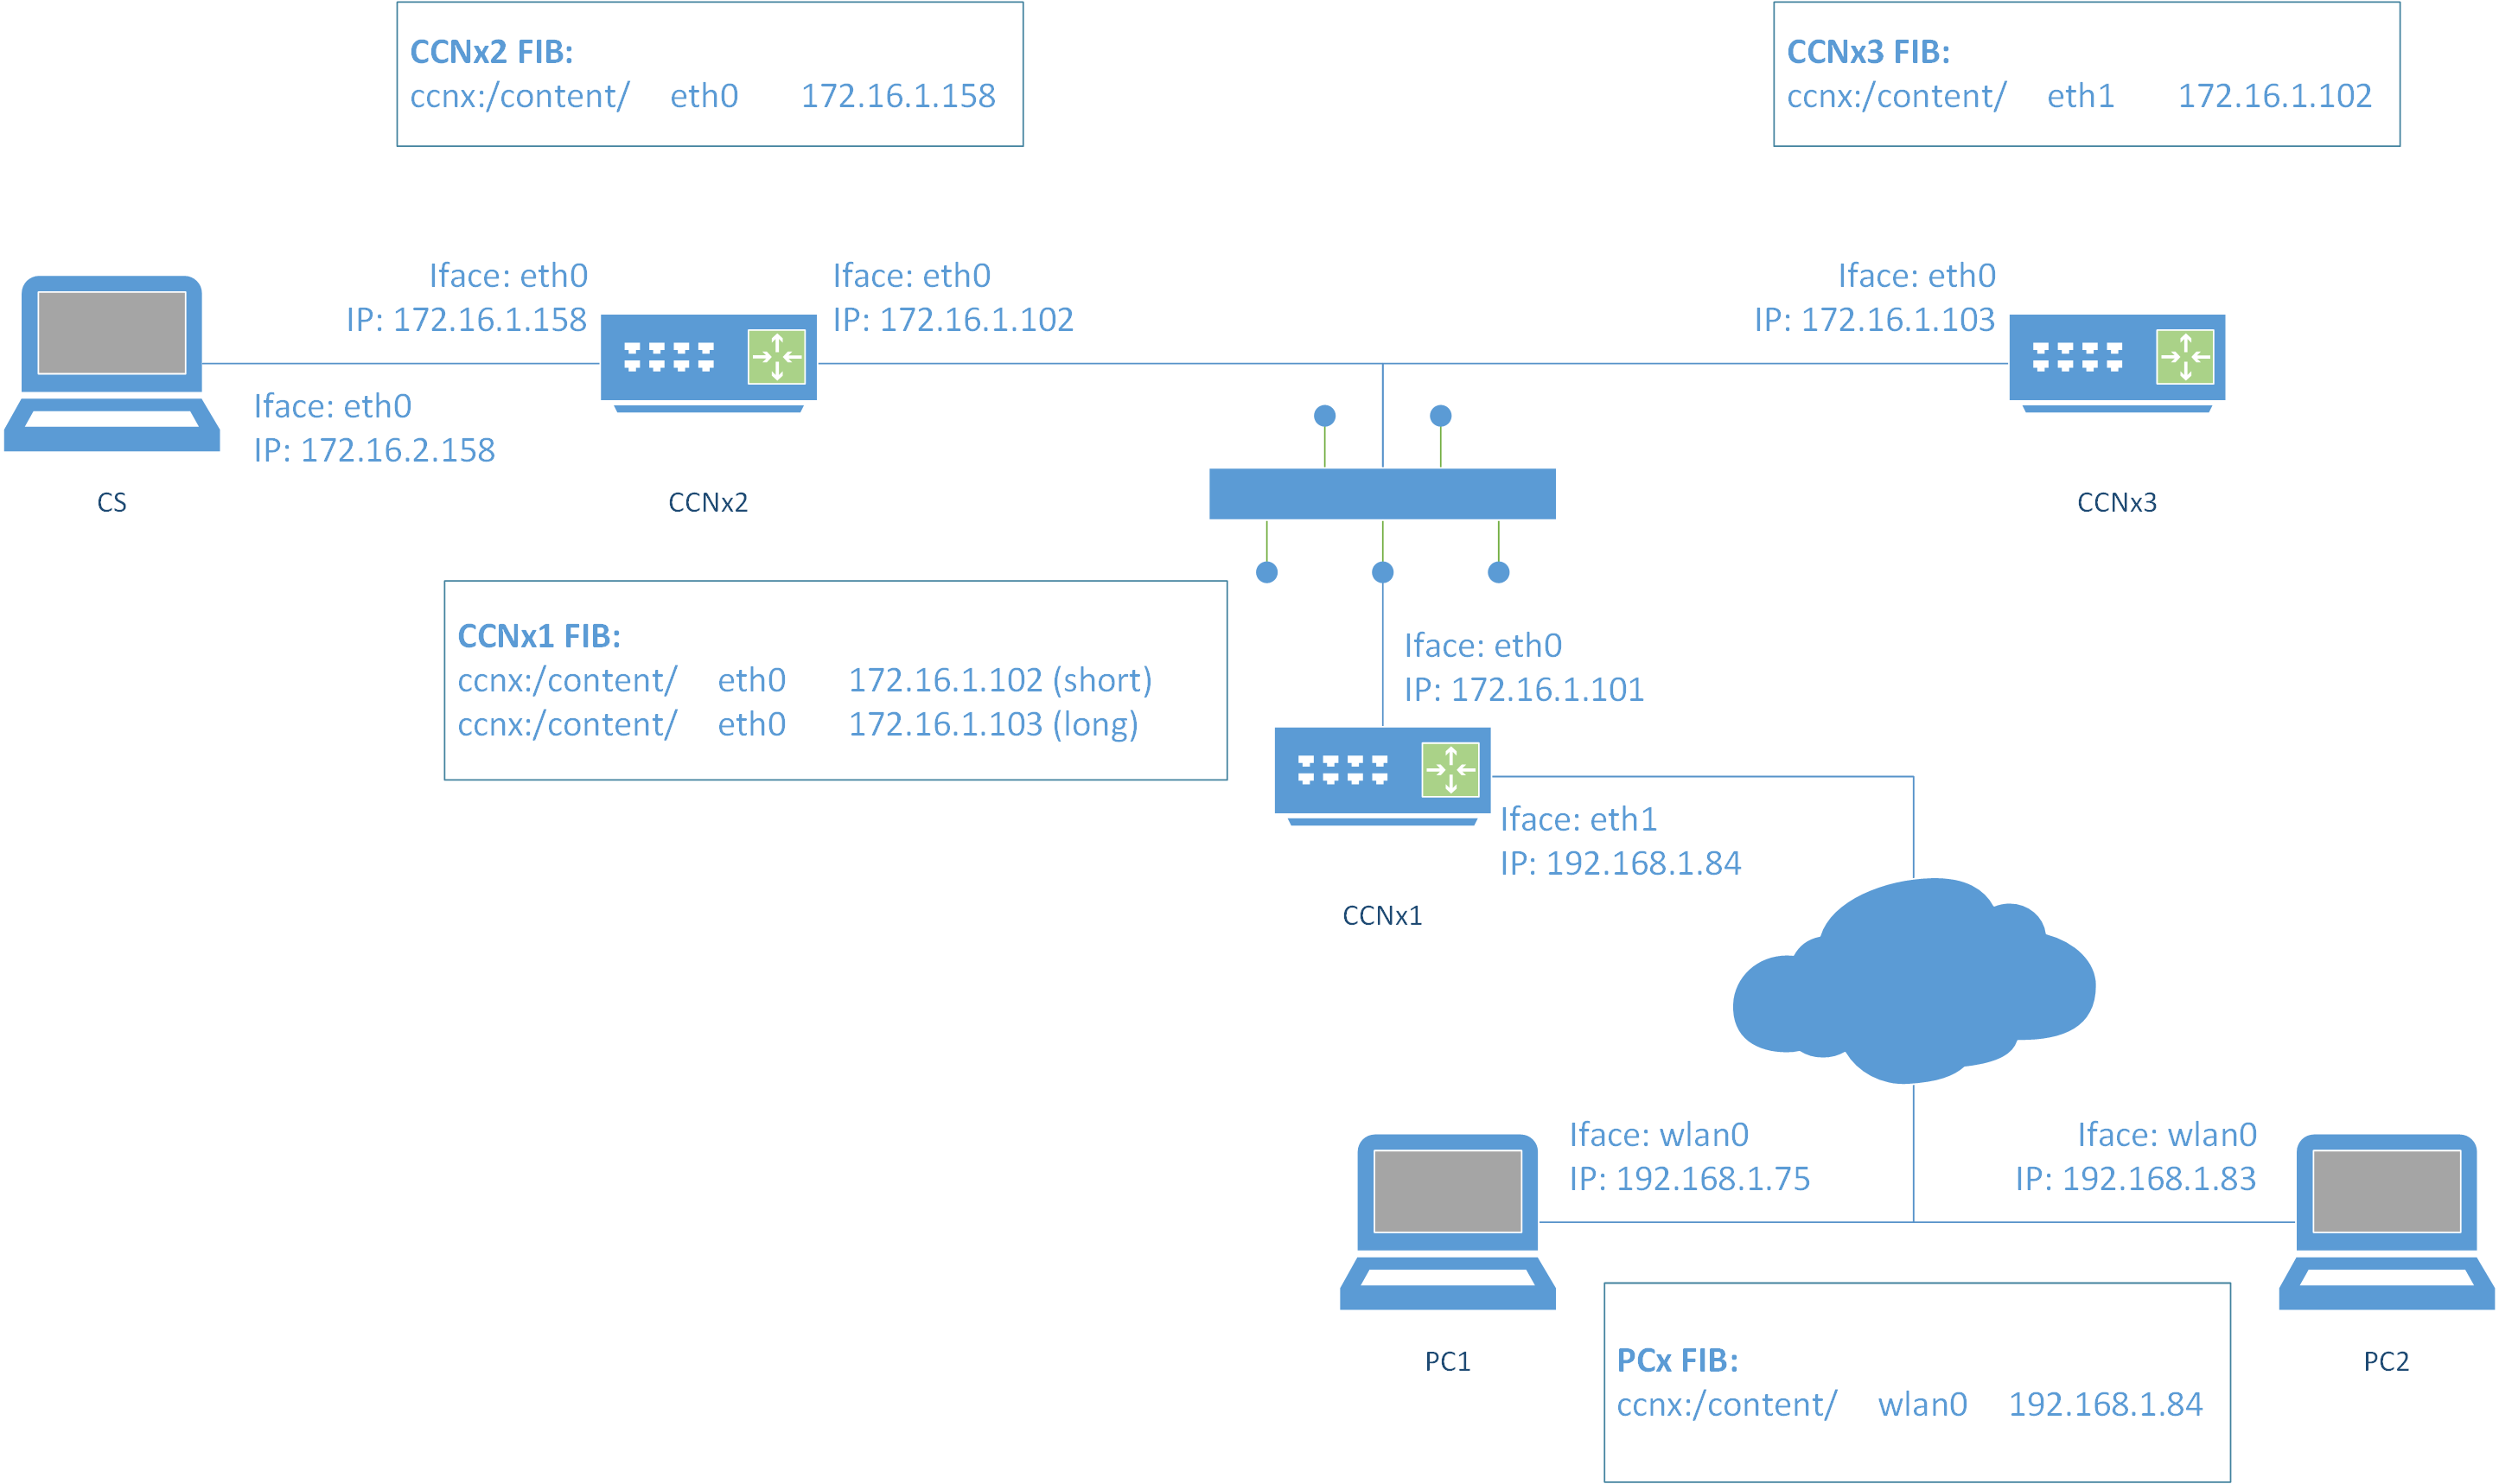
\includegraphics[width=0.80\textwidth]{figures/diag2.png}
    \cprotect\caption{Testbed arrangement for Test 2.3.}
    \label{fig:testbed-multiple-paths}

\end{figure}

The same type of content as that used in Test 2.1 (see 
Section~\ref{subsec:test-multihop-file}) is used, 
limited to a 5\,MB file. 
Again, the \verb+ccnr+ application is used at CS to host a CCNx file 
repository, while PC1 and PC2 retrieve the file using the \verb+ccngetfile+ 
application.\vertbreak 

Three subtypes of test are conducted: 

\begin{enumerate}

    \item PC1 and PC2 retrieve the content from CS via a short path, 
        via CCNx1 and CCNx2, in a non-overlapping fashion.
    \item PC1 and PC2 retrieve the content from CS via a long path, via 
        CCNx1, CCNx3 and CCNx2, in that order.
    \item PC1 and PC2 retrieve the content from CS with the INs configured 
        to forward packets via both short and long paths.

\end{enumerate}

The different paths are specified at the INs by adding manual entries to the 
FIB, using the \verb+ccndc+ command (see Section~\ref{subsubsec:fibs} for 
details). To test the influence of the order by which \verb+ccndc+ commands 
are ran, i.e. the order by which routing entries are put into the FIB, we 
first test a setting for which the `short path' is included first, followed 
by another setting for which the `long path' is included first. The same 
parameters as those measured in Tests 2.1 and 2.2 are evaluated in this case.

